\chapter{Ordinary Differential Equations}

A common differential equation we will encounter is a \emph{freefall problem}.
Here's an example:

\begin{figure}[H]
  \begin{center}
    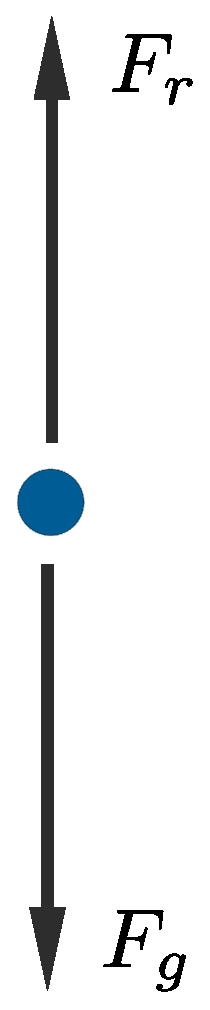
\includegraphics[width=1cm]{continuous/ode/freefall.eps}
  \end{center}
  \caption{A free-body diagram of an object in freefall.}
  \label{fig:freefall}
\end{figure}

Basic physics tells us that $\sum \vec F = m\vec a$,
where $m$ is the object's mass and $\vec{a}$ is the object's acceleration.
For our purposes, we will define $\vec F_g$ to be in the \emph{direction of increasing} $x$.
Based on these assumptions, we can state that
\[
  ma=\vec{F_g}+\vec{F_r}
  \]
Now, acceleration is the same as \emph{change in velocity,} so this is equivalent to
\[
  m\frac{\ud v}{\ud t}=mg - \gamma v
  \]
where $v$ is the object's velocity, $t$ is the time, $g$ is the acceleration of gravity near the surface of Earth, and $\gamma$ is the coefficient of friction for the air.

This is a \textbf{first-order linear ordinary differential equation}.
